\section{Numerical methods}\label{sec:FDTD}
This section will provide a brief introduction to physical modelling using FDTD methods, including details on stability and quality of the simulations based on these methods. In this section, $c$ is assumed constant.

\subsection{Discretisation}
In FDTD methods, the first step is the definition of a grid. The spatial variable can be discretised using $x_l = lh$ %(read: $x$ at spatial index $l$) 
with integer $l \in \{0, \hdots, N\}$. The grid spacing $h$ (in m) is the distance between adjacent grid points, and the total number of points covering the domain, including endpoints, is $N + 1$. Here, integer $N$ describes the total number of intervals between the grid points, and thus the total domain length is $L=Nh$.
%is described as
% \begin{equation}\label{eq:numberOfIntervals}
%     N = \lfloor L/h\rfloor,
% \end{equation}
% \SBcomment[Easier to write this as $h=L/N$, for integer $N$, so without a flooring operation.] \SWcomment[hmm.. this flooring operation is important for the comparison with $\Nfrac$ (fractional $N$) later on. Just clearly shows $N$ ``integerness" :)]\SBcomment[OK, but from the above, we don't have $L=Nh$, so the total domain length is off...well, at least for a standard domain!]\SWcomment[gotcha, I'll figure this out.. (something with \eqref{eq:orderOfCalcGrid} perhaps..)]
%with $\lfloor \cdot \rfloor$ denoting the flooring operation. 
The temporal variable can be discretised using $t_n = nk$ with positive integer $n$, time step $k = 1/f_\text{s}$ (in s) for sample rate $f_\text{s}$ (in Hz). The state variable $\ugen$ can then be approximated using 
$q_{l}^{n}\approxeq q(x=lh,t=nk)$. 
% $\ugen(x,t) \approx \ugen_l^n$, where grid function $\ugen_l^n$ approximates $\ugen$ at spatial index $l$ and time index $n$. %The total state at time index $n$ is then denoted as vector $\mathbf{u}^n$ with size $N+1$.

The following operators can then be applied to $\ugen_l^n$ to get the following approximations to the derivatives in Eq. \eqref{eq:1dwave}
\begin{subequations}\label{eq:operators}
    \begin{align}
         \delta_{tt}\ugen_l^n &= \frac{1}{k^2}\left(\ugen_l^{n+1}-2\ugen_l^n + \ugen_l^{n-1}\right)\;\;\approx\quad\frac{\partial^2\ugen}{\partial t^2}\label{eq:secondOrderTime}\ ,\\
         \delta_{xx}\ugen_l^n &= \frac{1}{h^2}\left(\ugen_{l+1}^n-2\ugen_l^n + \ugen_{l-1}^n\right)\quad\approx\quad \frac{\partial^2\ugen}{\partial x^2}\ .\label{eq:secondOrderSpace}
    \end{align}
\end{subequations}
Substituting these definitions into Eq. \eqref{eq:1dwave} yields the following finite-difference (FD) scheme
\begin{equation}\label{eq:FDS}
    \delta_{tt}\ugen_l^n = c^2 \delta_{xx}\ugen_l^n.
\end{equation}
%
Expanding the operators as in %the Eqs. in
\eqref{eq:operators} and solving for $\ugen_l^{n+1}$ yields the following update equation
\begin{equation}\label{eq:updateEq}
    \ugen_l^{n+1} = 2\ugen_l^n-\ugen_l^{n-1} + \lambda^2 \left(\ugen_{l+1}^n-2\ugen_l^n + \ugen_{l-1}^n\right),
\end{equation}
%saying that $\ugen$ at the next time index ($n+1$) can be calculated using only values of $\ugen$ at the current ($n$) and previous time indices ($n-1$).
which is suitable for direct software implementation. %This update can then be implemented in software, such as {\tt MATLAB} or {\tt C++}. 
Here,
\begin{equation}\label{eq:lambdaDef}
    \lambda = \frac{ck}{h}
\end{equation}
is referred to as the Courant number, constrained by numerical stability conditions, and also has an impact on the quality and behaviour of the simulation. This will be described in detail in Sections \ref{sec:stability} and \ref{sec:quality}.

In the FD scheme described in Eq. \eqref{eq:FDS}, the boundary locations are at $l = 0$ and $l = N$. Substituting these locations into Eq. \eqref{eq:updateEq} seemingly introduces the need of grid points outside of the defined domain, namely $\ugen_{-1}^n$ and $\ugen_{N+1}^n$. These can be referred to as \textit{virtual grid points} and can be accounted for using the boundary conditions in Eq. \eqref{eq:continuousBoundaries}. Discretising these yields
\begin{subequations}
    \begin{align}
        \ugen_0^n = \ugen_N^n &= 0, \quad\text{(Dirichlet)}\label{eq:discreteDirichlet}\\
        \delta_{x\cdot} \ugen_0^n = \delta_{x\cdot} \ugen_N^n &= 0, \quad \text{(Neumann)}\label{eq:discreteNeumann}
    \end{align}
\end{subequations}
where 
\begin{equation}
    \delta_{x\cdot}\ugen_l^n = \frac{1}{2h}\left(\ugen_{l+1}^n - \ugen_{l-1}^n\right)\quad \approx\quad \frac{\partial \ugen}{\partial x}
\end{equation}
is a second-order accurate approximation of the first-order spatial derivative. The Dirichlet condition in \eqref{eq:discreteDirichlet} says that the displacements of $\ugen$ at the boundary locations are always 0. In practice, this means that these grid points do not need to be updated and the spatial range of calculation for Eq. \eqref{eq:updateEq} then becomes $l \in \{1, \hdots, N-1\}$. If the Neumann condition is used, the boundary points do need to be updated as these are not necessarily $0$; rather, their `slope' is $0$. Eq. \eqref{eq:discreteNeumann} can then be expanded to yield defnitions for these virtual grid points
\begin{equation}\label{eq:neumannSolution}
    \ugen_{-1}^n = \ugen_1^n \quad \text{and} \quad \ugen_{N+1}^n = \ugen_{N-1}^n\,.
\end{equation}

Now that the full system is described, audio output at sample rate $f_\text{s}$ can be drawn from the state $\ugen_l^n$ in Eq. \eqref{eq:updateEq} at $0 < l < N$ (when using Dirichlet boundary conditions). %Though the output location does not change the behaviour of the system, it will determine the amplitude of different harmonic partials in the system output.

\subsection{Stability}\label{sec:stability}
Explicit FDTD methods for hyperbolic systems such as the 1D wave equation must necessarily satisfy a stability condition. In the case of the update in Eq. \eqref{eq:updateEq} it can be shown -- using von Neumann analysis \cite{Strikwerda1989} -- that the system is stable if
\begin{equation}\label{eq:CFL}
    \lambda \leq 1,
\end{equation}
which is referred to as the Courant-Friedrichs-Lewy (CFL) condition. The more closely $\lambda$ approaches this condition with equality, the higher the quality of the simulation (see Section \ref{sec:quality}) and if $\lambda = 1$, Eq. \eqref{eq:updateEq} yields an exact solution to Eq. \eqref{eq:1dwave}%(this is true for the 1D wave equation)
% (see Figures \ref{fig:dispersion}a and \ref{fig:dispersion}b)
. If $\lambda > 1$ the system will become unstable.
%  (see Figures \ref{fig:dispersion}a and \ref{fig:dispersion}b)
%
% \begin{figure}[t]
%     \centering
%     % \subfloat[]{\label{fig:lambda1}{ 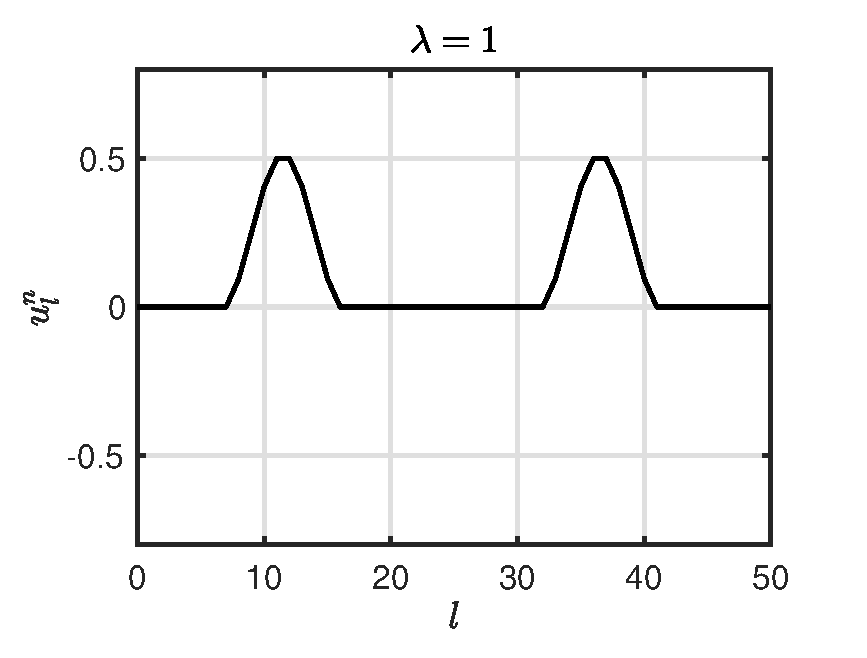
\includegraphics[width=0.3\textwidth]{Figures/ulnLambda1.eps}}}
%     % \subfloat[]{\label{fig:lambda0.9}{ 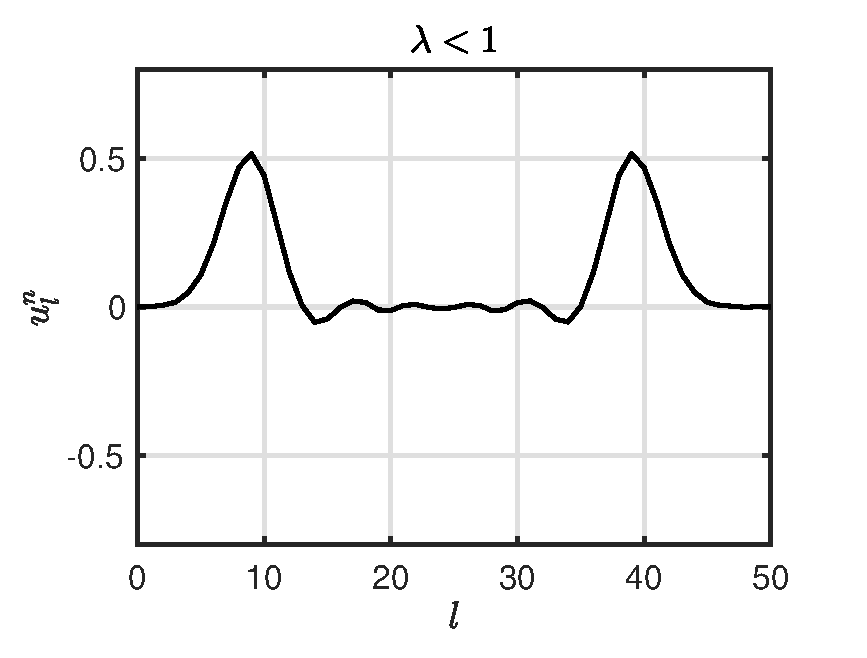
\includegraphics[width=0.3\textwidth]{Figures/ulnLambda09.eps}}}
%     % \subfloat[]{\label{fig:lambda1.001}{ 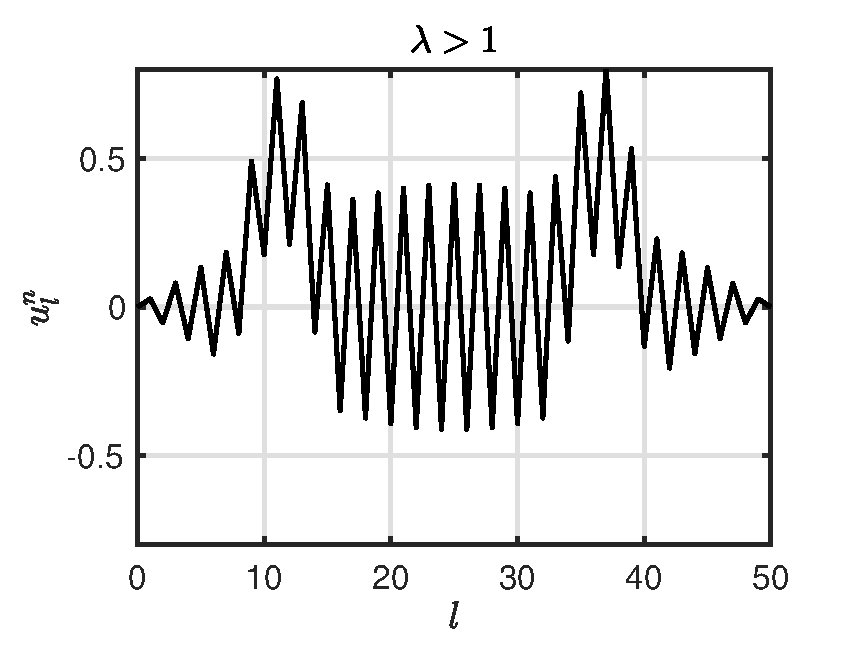
\includegraphics[width=0.3\textwidth]{Figures/ulnLambda1001.eps}}}
%     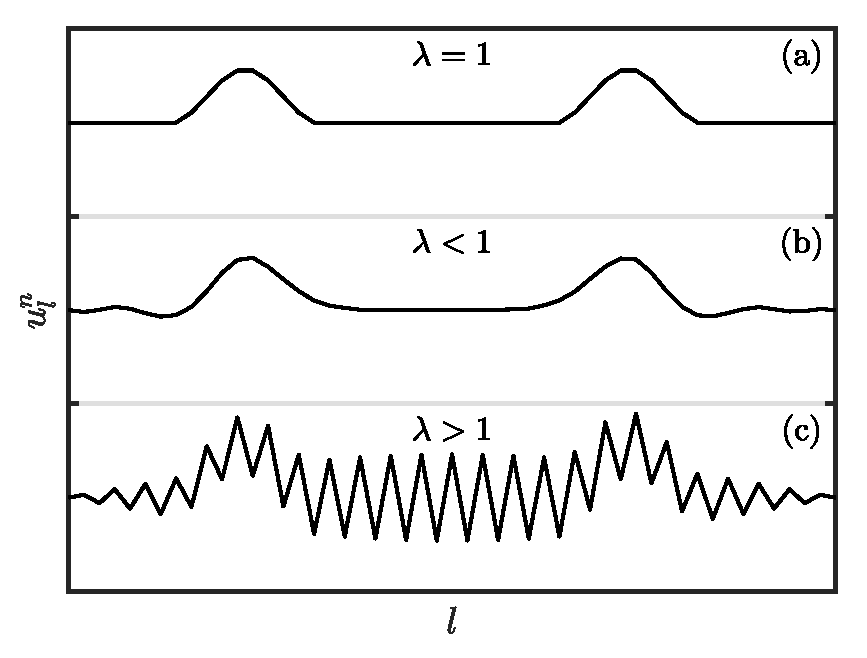
\includegraphics[width=0.8\columnwidth]{Figures/dispersionCompact.eps}
%     \caption{State $\ugen_l^n$ with $N = 50$ and $f_\text{s} = 44100$ visualised $\sim\!100$ samples after excitation. (a) If $\lambda = 1$, the solution is exact. (b) If $\lambda < 1$ dispersive behaviour shows. (c) If $\lambda > 1$ the CFL condition in Eq. \eqref{eq:CFL} is not satisfied and the system is unstable. \SWcomment[If $\ugen$ is used, don't forget to change in the figure!!]
%     \label{fig:dispersion}}
% \end{figure}
%
Recalling \eqref{eq:lambdaDef}, Eq. \eqref{eq:CFL} can be rewritten in terms of grid spacing $h$ to get
\begin{equation}\label{eq:stabilityCond}
    h \geq ck.
\end{equation}
This shows that the CFL condition in \eqref{eq:CFL} puts a lower bound on the grid spacing, determined by the sample rate and wave speed. Usually, the following steps are taken to calculate $\lambda$:
\begin{equation}\label{eq:orderOfCalcGrid}
    h := ck,\ \ N := \left\lfloor\frac{L}{h}\right\rfloor, \ \ h := \frac{L}{N}, \ \ \lambda := \frac{ck}{h},
\end{equation}
where $\lfloor \cdot \rfloor$ denotes the flooring operation. In other words, condition \eqref{eq:stabilityCond} is first satisfied with equality and used to calculate number of intervals $N$. Thereafter, $h$ is recalculated based on integer $N$ and used to calculate $\lambda$. The calculation of $\lambda$ in Eq. \eqref{eq:orderOfCalcGrid} can be compactly rewritten as
\begin{equation}\label{eq:compactLambda}
    \lambda = \frac{ck}{L}\cdot\left\lfloor\frac{L}{ck}\right\rfloor.
\end{equation}
The flooring operation causes the CFL condition in \eqref{eq:CFL} to not always be satisfied with equality and results in a reduced simulation quality described in the following section.

\subsection{Simulation Quality}\label{sec:quality}
%As mentioned above, the Courant number $\lambda$ decides the quality of the simulation. 
Choosing $\lambda < 1$ in Eq. \eqref{eq:updateEq} will decrease the simulation quality in two ways. Firstly, it will decrease the maximum frequency that the simulation is able to produce, i.e., it will decrease the bandwidth of the output sound of the system. 
%See Figure \ref{fig:bandWidths}.

% \begin{figure}[t]
%     \centering
%     % \subfloat[]{\label{fig:bandwidth1}{ 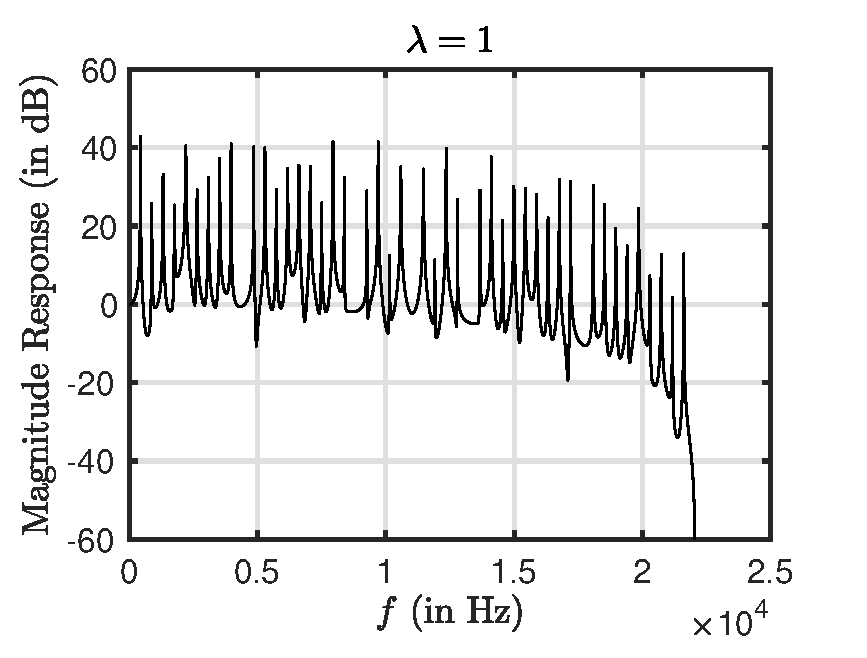
\includegraphics[width=0.3\textwidth]{Figures/bandwidthLambda1.eps}}}
%     % \subfloat[]{\label{fig:bandwidth09}{ 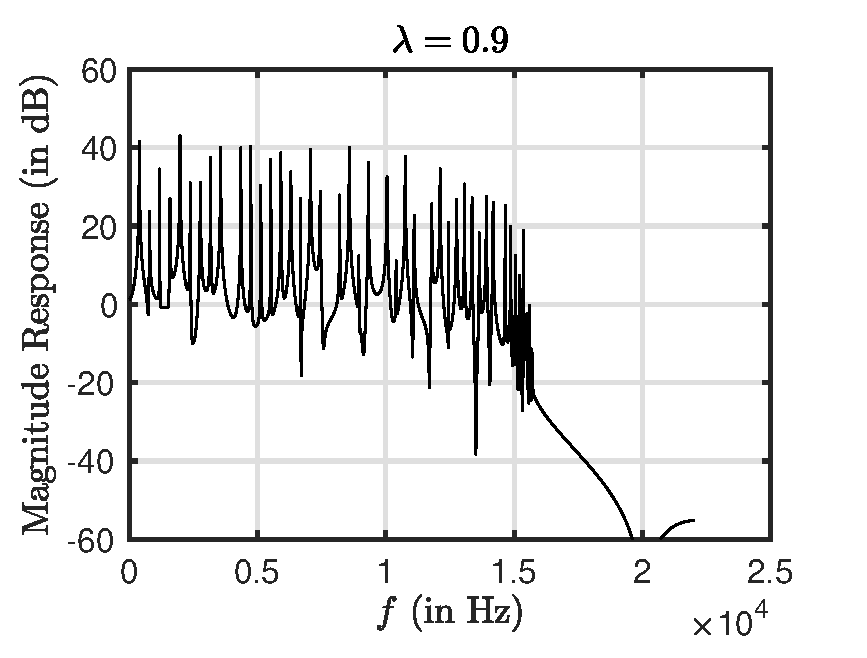
\includegraphics[width=0.3\textwidth]{Figures/bandwidthLambda09.eps}}}
%     % \subfloat[]{\label{fig:bandwidth05}{ 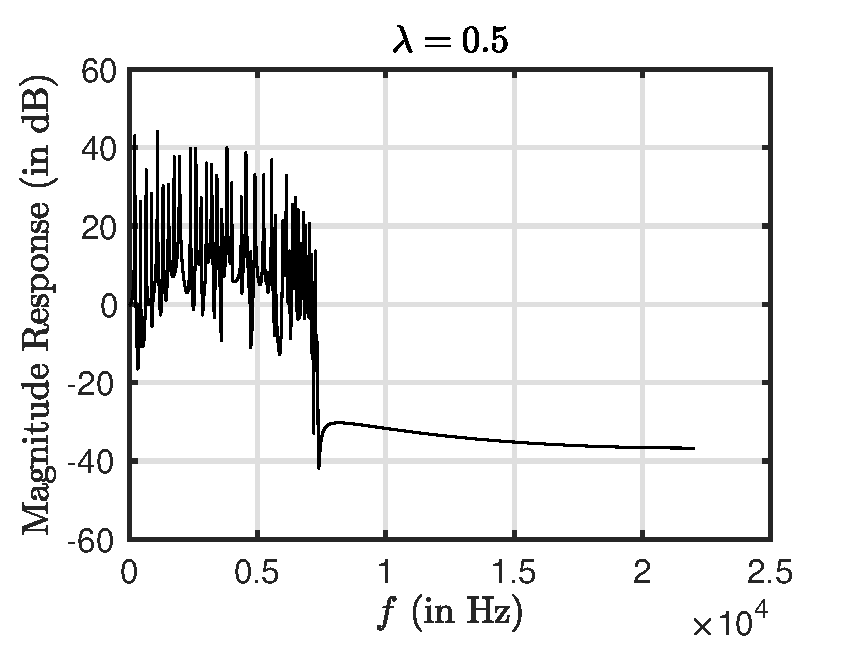
\includegraphics[width=0.3\textwidth]{Figures/bandwidthLambda05.eps}}}
%     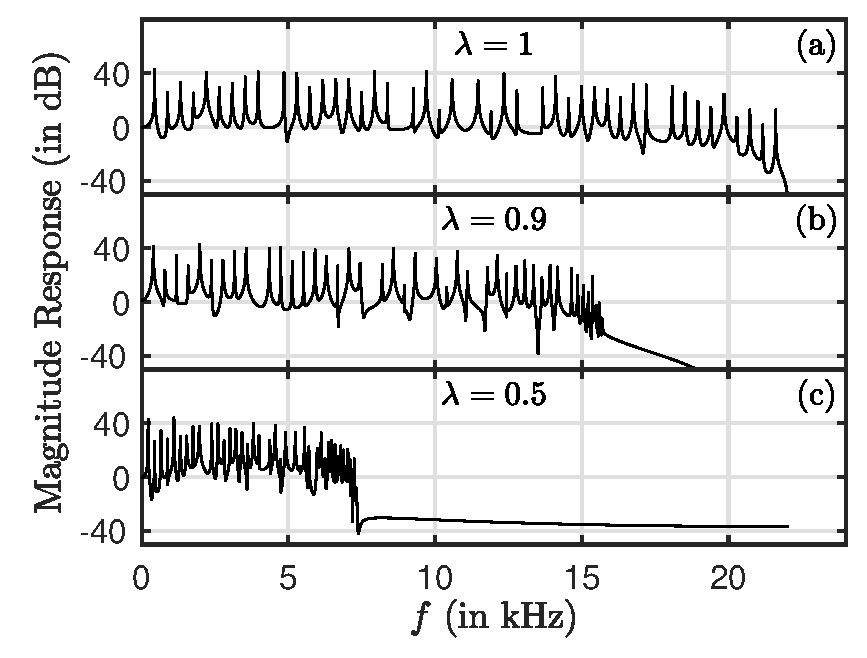
\includegraphics[width=0.9\columnwidth]{Figures/bandwidthCompact.eps}
%     \caption{Bandwidths of the simulation output %at $l = 16$ 
%     with $f_\text{s} = 44100$ Hz and 
%     %$N = 50$ excited with a raised cosine with a width of 5 at center-location $N = 25$. The Courant number is set to 
%     (a) $\lambda = 1$, (b) $\lambda = 0.9$ and (c) $\lambda = 0.5$. 
%     \label{fig:bandWidths}}
% \end{figure}
%
By analysing the scheme in Eq. \eqref{eq:updateEq}, it can be shown that the maximum frequency produced by the system can be calculated using $f_\text{max} = f_\text{s} \sin^{-1}(\lambda)/\pi$ \cite[Chap. 6]{bilbao2009}.
% \begin{equation}\label{eq:fmax}
%     f_\text{max} = \frac{f_\text{s}}{\pi} \sin^{-1}(\lambda).
% \end{equation}
% shown in Figure \ref{fig:bandWidthFormula}.
%
Note that only a small deviation of $\lambda$ from condition \eqref{eq:CFL} leads to a large reduction in output bandwidth.
%
% \begin{figure}
% %% \reprintcolumnwidth is the same in preprint and reprint for
% %% ease of use for authors:
% \includegraphics[width=0.8\reprintcolumnwidth]{bandwidthPlot}
% \caption{\label{fig:bandWidthFormula}{The effect of the Courant number $\lambda$ on the output bandwidth. \SWcomment[This figure should probably be much more compact, if not removed altogether.]}}
% \end{figure} 
Secondly, choosing $\lambda < 1$ causes numerical dispersion. %See Figures \ref{fig:dispersion}b and \ref{fig:bandWidths}. 
Harmonic partials become unnaturally closely spaced at higher frequencies (i.e. spurious inharmonicity increases) as $\lambda$ decreases, which is generally undesirable.

%\SWcomment[can cut this paragraph $\rightarrow$] Apart from the recalculation of $\lambda$ due to the flooring operation in Eq. \eqref{eq:orderOfCalcGrid}, a reason that one would choose $\lambda < 1$ could be to decrease the total number of grid points used in the simulation by increasing $h$. This makes the simulation less computationally expensive, while keeping a desired wave speed $c$ and time step $k$. For 1-dimensional systems such as the 1D wave equation, this is rarely necessary.
